\documentclass[../dissertation.tex]{subfiles}
 
\begin{document}

\section{Appendix B: Example Stimuli for Sloutsky Statistical Density Task} \label{appendixB}

\subsection{Sparse stimuli}

\begin{figure}[H]
\begin{center}
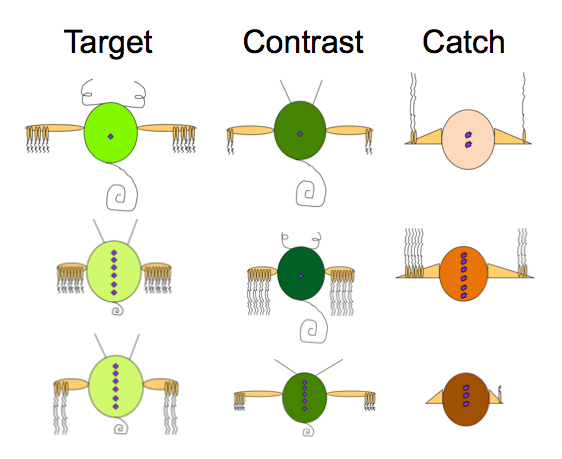
\includegraphics[scale=0.5]{bug_examples}
\caption[Example stimuli for supervised-sparse blocks]{Example stimuli for supervised-sparse blocks. Bugs varied on body color, tail size, wing length, number of fingers, finger length, dot number, and antennae shape.}
\vspace{-10pt}
\label{bugs}
\end{center}
\end{figure}

\begin{figure}[H]
\begin{center}
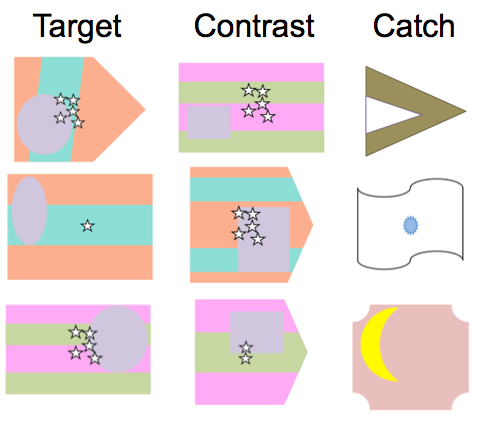
\includegraphics[scale=0.4]{flag_examples}
\caption[Example stimuli for unsupervised-sparse blocks]{Example stimuli for unsupervised-sparse blocks. Flags varied on shape, color, stripe direction, number of stars, overlay shape, overlay position, and overlay size.}
\vspace{-10pt}
\label{flags}
\end{center}
\end{figure}

\subsection{Dense stimuli}

\begin{figure}[H]
\begin{center}
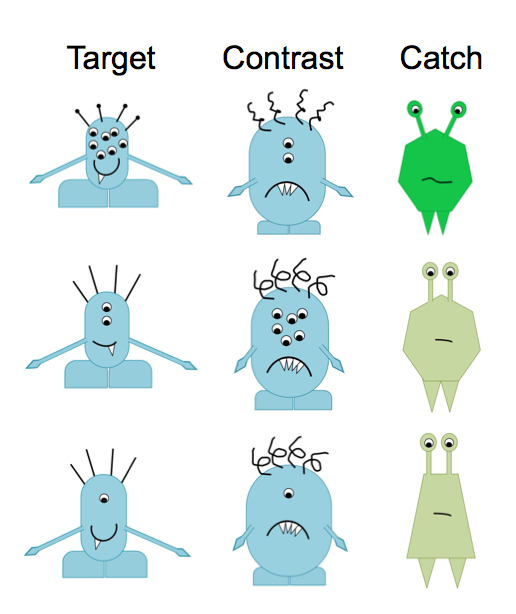
\includegraphics[scale=0.4]{alien_examples}
\caption[Example stimuli for unsupervised-dense blocks]{Example stimuli for unsupervised-dense blocks. Aliens varied on body size, arm length, foot size, number of teeth, smiling/frowning, hair shape, and number of eyes.}
\vspace{-10pt}
\label{aliens}
\end{center}
\end{figure}

\begin{figure}[H]
\begin{center}
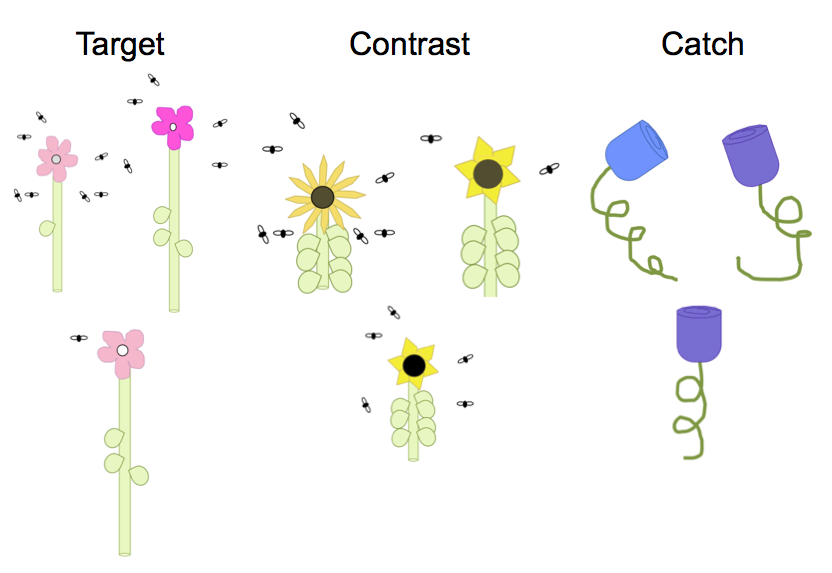
\includegraphics[scale=0.4]{flower_examples}
\caption[Example stimuli for supervised-dense blocks]{Example stimuli for supervised-dense blocks. Flowers varied on petal shape, petal color, stem length, number of leaves, center size, center color, and number of bugs.}
\vspace{-10pt}
\label{flowers}
\end{center}
\end{figure}



\end{document}
